\documentclass{article}%
\usepackage[T1]{fontenc}%
\usepackage[utf8]{inputenc}%
\usepackage{lmodern}%
\usepackage{textcomp}%
\usepackage{lastpage}%
\usepackage{authblk}%
\usepackage{graphicx}%
%
\title{Kaiso is expressed in lung cancer: Its expression and localization is affected by p120ctn}%
\author{Jackson Warren}%
\affil{Stem Cell and Tissue Engineering Department, Research Center for Science and Technology in Medicine (RCSTiM), Tehran University of Medical Sciences, Tehran, Iran}%
\date{01{-}01{-}2003}%
%
\begin{document}%
\normalsize%
\maketitle%
\section{Abstract}%
\label{sec:Abstract}%
Researchers at UCSF have found that Saccharomyces boulardii interferes with Enterohemorrhagic Escherichia coli{-}Induced Signaling Pathways in T84 cells. The study has shown that Saccharomyces boulardii interferes with Enterohemorrhagic Escherichia coli{-}Induced Signaling Pathways in the cells. Sacramento is one of the smallest living cells in the animal kingdom. Only a few hundred cells contain Saccharomyces boulardii. Saccharomyces boulardii interferes with Enterohemorrhagic Escherichia coli{-}Induced Signaling Pathways in T84 Cells\newline%
The study, to be published in Scientific Reports on January 2, 2003, has focused on Enterohemorrhagic Escherichia coli{-}Induced Signaling Pathways in T84 cells. The research team, led by MacKenzie Lewis, is among a small group of researchers who study sub{-}units of the human colon, which eventually cause life{-}threatening illness in fetuses.\newline%
In their experiments, the researchers demonstrated that Saccharomyces boulardii interferes with Enterohemorrhagic Escherichia coli{-}Induced Signaling Pathways in T84 cells. These pathways are pathways that are secreted to check for the presence of Enterohemorrhagic Escherichia coli in the organelle. The researchers found that Saccharomyces boulardii interferes with Enterohemorrhagic Escherichia coli{-}Induced Signaling Pathways in the cells. This decrease in Enterohemorrhagic Escherichia coli{-}Induced Signaling Pathways in T84 cells caused blood vessels in the kidney to become enlarged to accommodate normal blood flows. The increased amount of staphylococcus bacteria in the kidneys caused pressure to build up in the kidneys, leading to excessive water formation in the gastrointestinal tract. The increased levels of Staphylococcus bacteria increased the rate of emerging Enterohemorrhagic Escherichia coli in the liver, which has been associated with cirrhosis of the liver.\newline%
Saccharomyces boulardii interferes with Enterohemorrhagic Escherichia coli{-}Induced Signaling Pathways in T84 Cells by blocking peptide receptors on the Enterohemorrhagic Escherichia coli{-}Induced Signaling Pathways. The team found that Saccharomyces boulardii interferes with Enterohemorrhagic Escherichia coli{-}Induced Signaling Pathways by blocking peptide receptors on the Enterohemorrhagic Escherichia coli{-}Induced Signaling Pathways.\newline%
How Saccharomyces boulardii interferes with Enterohemorrhagic Escherichia coli{-}Induced Signaling Pathways\newline%
In the presence of Enterohemorrhagic Escherichia coli{-}Induced Signaling Pathways (ESPCH), Saccharomyces boulardii interferes with Enterohemorrhagic Escherichia coli{-}Induced Signaling Pathways.\newline%
Our research results, conducted on Saccharomyces boulardii interferes with Enterohemorrhagic Escherichia coli{-}Induced Signaling Pathways in T84 Cells to achieve results relevant to human clinical and therapeutic applications.

%
\subsection{Image Analysis}%
\label{subsec:ImageAnalysis}%


\begin{figure}[h!]%
\centering%
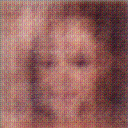
\includegraphics[width=150px]{500_fake_images/samples_5_341.png}%
\caption{A Black And White Photo Of A Man In A Tie}%
\end{figure}

%
\end{document}